%%% Fiktivní kapitola s ukázkami tabulek, obrázků a kódu

\chapter{Implementace projektu}
V předchozí kapitole jsme prošli funkční požadavky, očekávané od vyvíjeného
souboru programů. Následuje rozbor jednotlivých modulů, které vznikly při
vlastní implementaci. 

\paragraph{Programovací jazyk}
Celý projekt je napsána v programovacím jazyce \textbf{Python}. Cílem projektu
je vytvořit čitelnou rozšířitelnou platformu, která bude uživateli jednoduše
dostupná. Pokud uživatel bude mít potřebu vytvořené moduly jakkoli měnit nebo
rozšiřovat, Python toto bez problémů umožní. Jednoduchá čitelnost Pythonu
spojená s rychlostí, jakou mohou být prováděny iterace změn, bez potřeby
zdlouhavého překladu celé knihovny, se nám zdají býti dostatečně užitečné
vlastnosti volbu Pythonu jako jazyka pro tento projekt.

\paragraph{Struktura projektu}

%TODO: Change basic imp_graph
\begin{figure}[!htb]
    \centering
    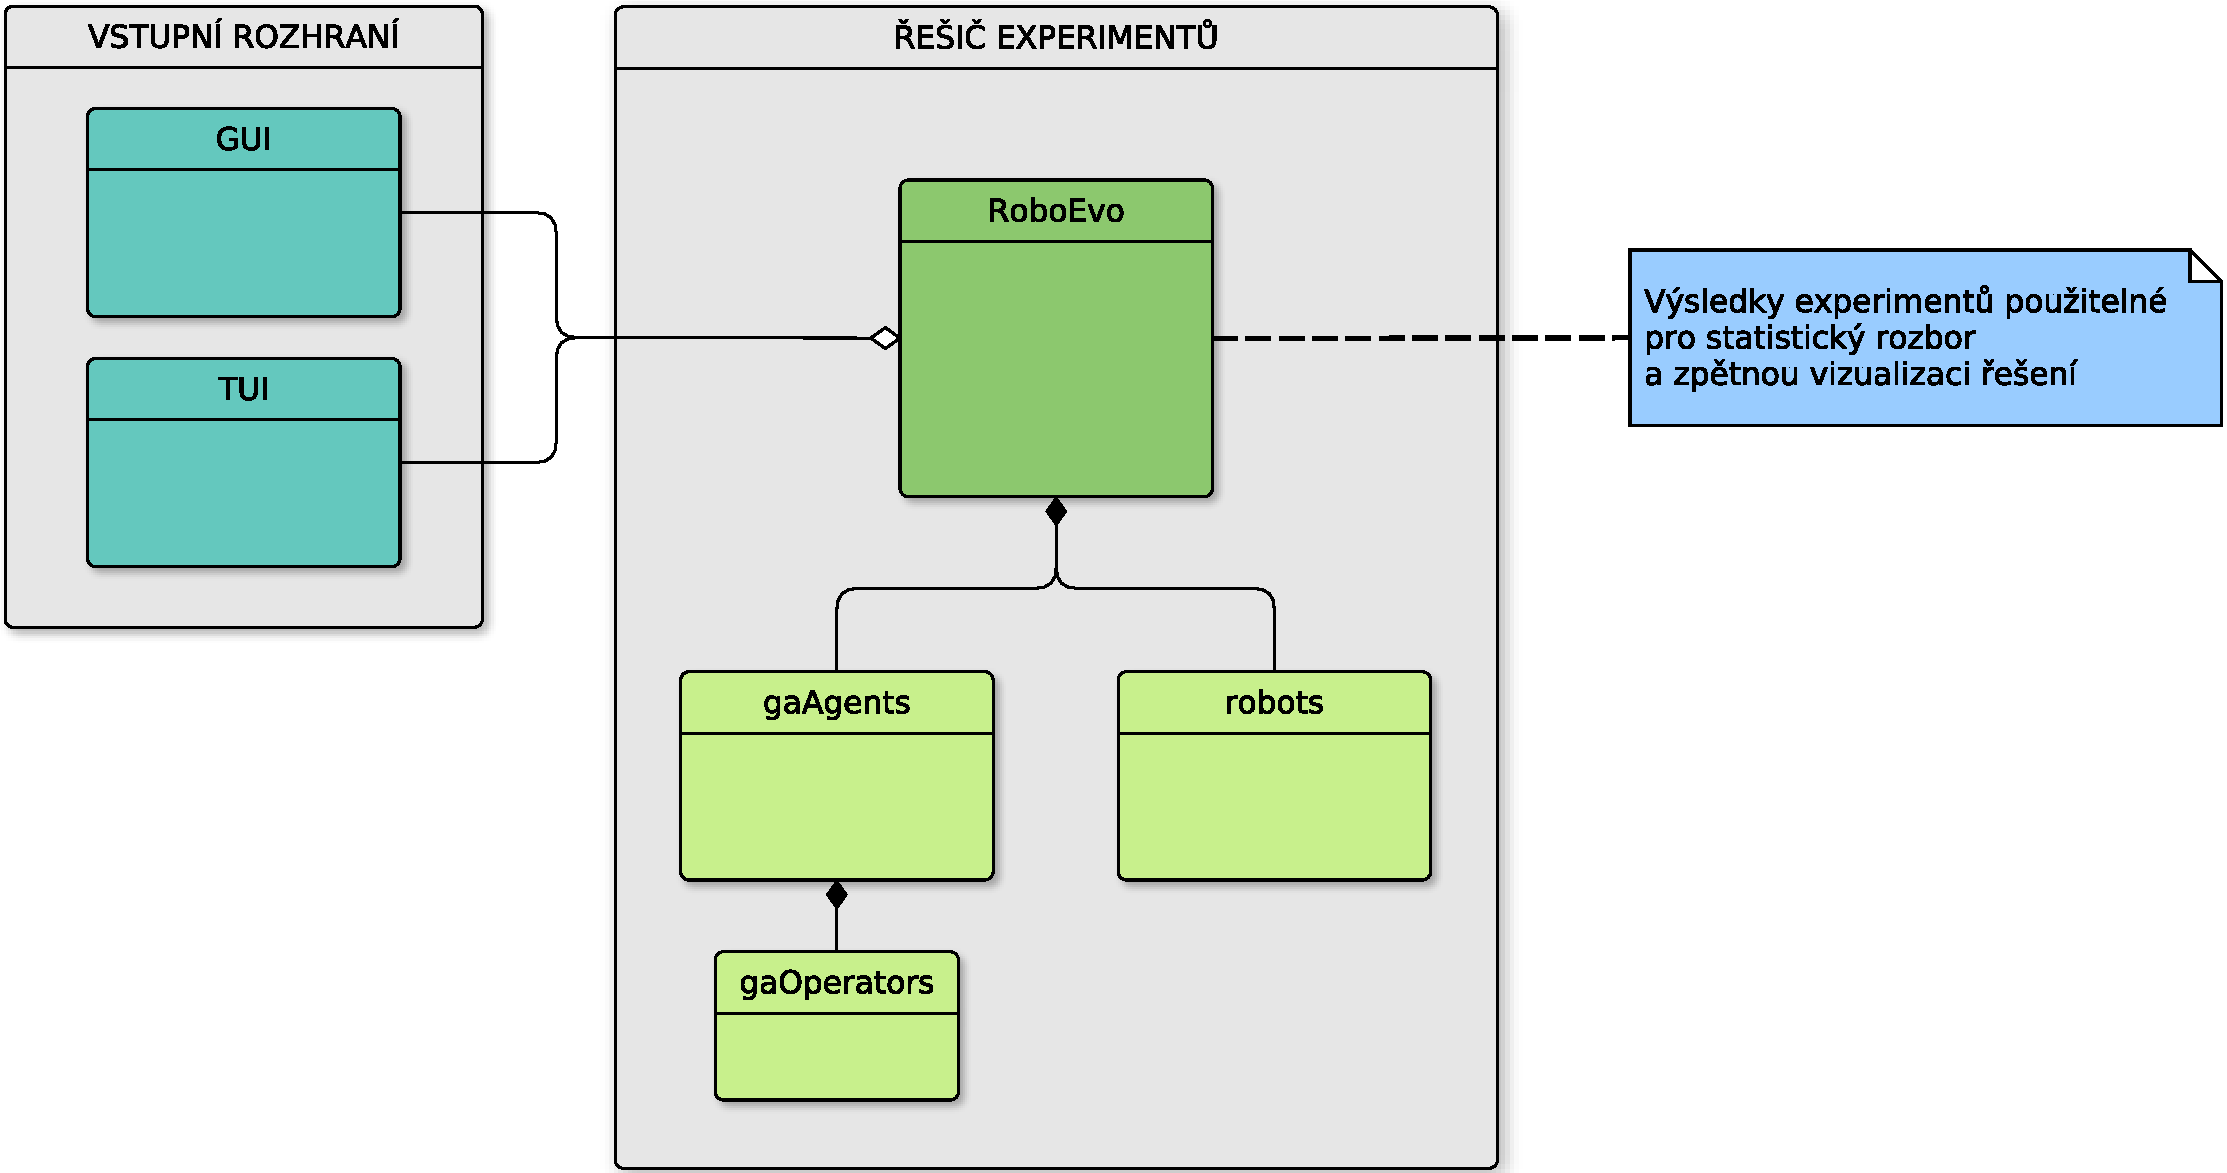
\includegraphics[width=1\textwidth]{../img/BP_imp_graph.pdf}
    \caption{Struktura projektu}
    \label{fig:struktura}
\end{figure}

Obrázek \ref{fig:struktura} popisuje na jaké části je projekt rozdělen.
Centrální částí je modul \emph{RoboEvo}, pomocí kterého knihovna provádí
evoluční experimenty. Tento modul se pro přehlednost a rozšířitelnost kódu
skládá z několika menších částí -- \emph{gaAgents} (popisující agenty a vlastní
genetické operátory) a \emph{robots} (udržující jednotný způsob přístupu k
různým robotům). 

Jak popisují funkční požadavky (v sekci \ref{Specifikace-funkčnípožadavky}),
projekt umožňuje několik možných způsobů práce s naší knihovny. Dva základní
možné přístupy jsou za pomoci grafického, nebo textového rozhraní. Tyto
přístupy jsou v projektu rozděleny do \emph{GUI} (\emph{Graphical User
Interface}) a \emph{TUI} (\emph{Text-based User Interface}) modulů. Uživatel,
který bude chtít pracovat s kódem části knihovny zaměřené na vytváření a
provádění experimentů s evolučním vývojem, se dále může zaměřit na hlavní modul
\emph{RoboEvo} (a s ním spojené pomocné moduly).

\paragraph{} 
Dále v této kapitole v sekci \ref{imp:roboevo} popíšeme centrální modul
\emph{RoboEvo} pracující s několika dalšími pomocnými moduly, jejichž
implementace popíšeme v dalších oddílech. Popíšeme třídu agentů v oddílu
\ref{imp:gaAgents}. Implementace vlastních genetických operátorů se nachází v
oddílu \ref{imp:gaOperators}. Vlastní modul \emph{robots} propojující roboty ze
simulátoru \emph{MuJoCo} (MuJoCo popsáno v základních pojmech v oddílu
\ref{MuJoCo}) s ostatními třídami je vysvětlena (v oddílu \ref{imp:robots}). V
sekci \ref{imp:experimentsetter} předvedeme třídu \texttt{Experiment} modulu
\emph{experiment\_setter}, sloužící k uchování a předvolbě parametrů pro
experimenty, usnadňující tak provádění většího množství experimentů. Jako
poslední si představíme moduly umožňující uživateli práci s knihovnou buď
pomocí grafického prostředí (v sekci \ref{imp:GUI}), nebo pomocí příkazové
řádky (v sekci \ref{imp:TUI}). 

\section{RoboEvo a pomocné moduly}
V této sekci popíšeme hlavní modul \emph{RoboEvo} a jeho pomocné moduly
\linebreak \emph{gaAgents}, \emph{gaOperators} a \emph{robots}. Soubor těchto
modulů tvoří hlavní část celého projektu, obsahující celý proces umožňující
provádění evolučních experimentů s roboty. Vybrané rozdělení modulů bylo
vytvořeno pro zlepšení čitelnosti a zjednodušení rozšiřování kódu, kde nyní
každý modul zprostředkovává velmi specifickou roli v procesu evolučního vývoje,
a tudíž je pro uživatele jednoduché tyto části upravovat. Tato část projektu je
zároveň zcela oddělena od zpracování uživatelského vstupu, který do hlavního
modulu vstupuje z vnějších modulů až ve chvíli zahájení experimentu. 

\subsection{Modul RoboEvo} \label{imp:roboevo}
Modul \emph{RoboEvo} je centrální modul tohoto projektu, sloužící pro spouštění
a běh experimentů s evolučním vývojem robotů. 

Každý experiment se skládá z několika nezávislých částí. Experiment může
využívat různé typy evolučních agentů s různými genetickými operátory a může se
snažit vyvíjet různé typy robotů. Jak bylo zmíněno výše, tyto částí jsou pro
přehlednost, čitelnost a rozšířitelnost kódu oddělené do vlastních menších
implementací, rozšiřující hlavní modul (jednotlivé implementace budou popsány v
dalších oddílech). 

\paragraph{Implementace modulu \emph{RoboEvo}}
Tento modul obsahuje funkce sloužící jak k inicializaci evolučních experimentů,
tak k samotnému běhu evolučních algoritmů, včetně propojení s knihovnou
\emph{Gymnasium} od Farama Foundation (popsáno v sekci \ref{Simulátory -
Porovnání}), zprostředkovávající simulaci fyzikálního prostředí pro testování
jedinců.

Hlavní funkcí, která z vnějšího vstupního prostředí (např. \emph{GUI},
\emph{TUI}, vlastní modul uživatele) přijímá parametry pro spuštění
experimentů, je funkce \linebreak\texttt{run\_experiment}. Povinným parametrem
této funkce jsou parametry \linebreak experimentu, které jsou pro zapouzdření
vloženy do jednoduché třídy \linebreak\texttt{ExperimentParams} (modul
\emph{experiment\_params}) obsahující následující hodnoty:

%TODO: LOOK AT BLACK BARS FOR LINEBREAKS \linebreak

%TODO: care for params changes
\begin{itemize}
    \item \texttt{robot} -- zvolený robot z modulu \texttt{robots},
    \item \texttt{agent} -- zvolený agent z modulu \texttt{gaAgents},
    \item \texttt{ga\_population\_size} -- velikost populace jedinců v
        evolučním algoritmu,
    \item \texttt{ga\_generation\_count} -- počet generací, po které bude
        evoluční algoritmus běžet,
    \item \texttt{show\_best} -- příznak určující, zda po doběhnutí evolučního
        algoritmu \\chceme v simulovaném prostředí zobrazit řešení nejlepšího
        jedince,
    \item \texttt{save\_best} -- příznak určující, zda po doběhnutí evolučního
        algoritmu \\chceme uložit nejlepšího jedince,
    \item \texttt{save\_dir} -- cesta ke složce, kam chceme uložit data z běhu
        evolučního algoritmu (pokud neexistuje, je složka automaticky vytvořena
        po doběhnutí algoritmu),
    \item \texttt{show\_graph} -- příznak určující, zda je při běhu algoritmu
        vykreslován graf zobrazující fitness hodnoty (min, mean a max) v
        jednotlivých generacích,
    \item \texttt{note} -- případná poznámka, kterou může uživatel speciálně
        odlišit název dat, ukládaných po doběhnutí algoritmu.
\end{itemize}

Funkce \texttt{run\_experiment} zpracovává tyto parametry a zajišťuje vše
potřebné pro běh experimentu. V přípravě probíhá spouštění výpočetních
jednotek pro paralelizaci testovacího prostředí (umožňující ohodnocení
populace jedinců paralelně). Následně proběhne spuštění evolučního algoritmu se
zvolenými parametry, po kterém funkce uloží data vygenerovaná evolučním
algoritmem -- fitness hodnoty jedinců v každé generaci, celá
populace jedinců z poslední generace a (volitelné) nejlepší řešení na konci
experimentu. Tato data jsou uložená do složky, dostupné na cestě popsané v
parametru \texttt{save\_dir}.

\paragraph{Běh evolučního algoritmu}
Funkce \texttt{run\_experiment} zajišťuje spuštění evolučního algoritmu se
zvolenými parametry. Samotný běh evolučního algoritmu je poté zajištěn funkcí
\texttt{run\_evolution}. V rámci této funkce provádíme všechny kroky evolučního
algoritmu (jak byly popsány v základních pojmech evolučních algoritmů v sekci
\ref{Evoluční algoritmy}). Navíc zde pro jedince vytváříme simulační prostředí,
ve kterých budou jedinci testováni při výpočtu fitness.

Po výpočtu fitness přichází na řadu genetické operátory, které jsou vždy
specifické pro zvolený evoluční algoritmus. V naší implementaci jsou zvolené
operátory specifikované v třídě agenta. Podrobněji třídu agentů
popíšeme v dalším oddíle \ref{imp:gaAgents}.

V rámci této funkce se zároveň sbírají důležitá data o vývoji fitness hodnot
napříč všemi generacemi a pokud to uživatel povolil, jsou aktuální data v
průběhu algoritmu vykreslována do jednoduchého grafu.

\subsection{Modul \emph{gaAgents}} \label{imp:gaAgents}
Modul \emph{gaAgents} je kolekcí několika tříd popisující agenty využívané
evolučními algoritmy. Každá třída agenta povinně obsahuje několik funkcí, které
specifikují jak vypadá genotyp jedinců vytvořených podle tohoto agenta, jakým
způsobem se generuje populace takových jedinců, jaké genetické operátory budou
při evolučním vývoji použité a jakým stylem probíhá transformace genotypu
jedince na nastavení odpovídajících aktuátorů robota. Agent zároveň uchovává
informaci o zvoleném typu evoluce, který určuje, zda evoluční algoritmus může
vyvíjet řízení robota, jeho morfologii nebo obojí.

Agent pro evoluční algoritmus vytváří jedince, jejichž genotyp se skládá ze
dvou vektorů. První z vektorů vždy obsahuje hodnoty, pomocí kterých agent
generuje na základě vstupu z testovacího prostředí odpovídající nastavení pro
aktuátory robota. Druhý z vektorů obsahuje hodnoty popisující délku těch částí
těla robota, u kterým jsme povolili jejich vývoj pomocí evolučního algoritmu.
Pokud jsme nepovolili vývoj žádné části těla, tento vektor zůstane prázdný.

\paragraph{Třída agenta}
Hlavní třídou tohoto modulu, tvořící šablonu pro všechny další definované
agenty, je třída \texttt{BaseAgent}. Všechny třídy popisující agenty mají
povinnost odvozovat od této třídy základního agenta. Součástí této třídy je
několik abstraktních metod (metody, které odvozená třída má povinnost
implementovat, aby byla použitelná). Výčet abstraktních metod agenta:

\begin{enumerate}[a)]
    \item metody využívané evolučním algoritmem:
        \begin{itemize}
            \item \texttt{generate\_population(population\_size)} -- metoda
                vytvářející populaci jedinců požadované velikosti,
            \item \texttt{get\_action(individual, step)} -- metoda
                zprostředkovávající transformaci části genotypu jedince
                (kterou funkce získá z parametru \texttt{individual}) na
                nastavení pro aktuátory daného robota na základě vstupu z
                testovacího prostředí (simulační krok v testovacím prostředí --
                z parametru \texttt{step}),
            \item \texttt{selection(population, fitness\_values)} -- genetický
                operátor -- metoda s parametry populace jedinců a jejich
                fitness hodnotami, která nějakým způsobem (s využitím
                genetických operátorů selekce) vybere jedince a vrátí jejich
                seznam,
            \item \texttt{crossover(population)} -- genetický operátor --
                metoda s parametrem populaci jedinců (označující skupinu
                rodičů), na které provede křížení genotypů a vrátí vytvořenou
                skupinu potomků,
            \item \texttt{mutation(population)} -- genetický operátor -- metoda
                do které jako parametr vstoupí skupina jedinců (potomků
                křížení), na kterých provede mutaci genotypu a vrátí
                zmutované potomky,
        \end{itemize}
    \item metody využívané pro vstupní rozhraní:
        \begin{itemize}
            \item \texttt{for\_GUI(...)} -- metoda, která vytváří agenta s
                výchozím nastavením(využíván při prezentaci agenta v
                \emph{GUI}),
            \item \texttt{description()} -- metoda, do které můžeme vložit
                text, sloužící jako rozsáhlejší popisek agenta v \emph{GUI}.
        \end{itemize}
\end{enumerate}

Využití abstraktních metod se pro tuto implementaci hodí, protože tímto
způsobem můžeme v experimentech jednoduše zaměňovat typy využívaných
agentů a měnit tak průběh evolučního vývoje. 

\paragraph{Vlastní agent}
Uživatel pak může jednoduše přidávat vlastní agenty, vytvořením třídy odvozené
od třídy \texttt{BaseAgent} a implementováním potřebných metod. Pro
zjednodušení tohoto procesu, uživatel nemusí vlastnoručně programovat všechny
tyto metody, ale může využít připravené genetické operátory, implementované v
pomocném modulu \emph{gaOperators}, který si představíme v následujícím oddílu
\ref{imp:gaOperators}. Pokud uživatel nenajde takovou funkci, která by přesně
odpovídala jeho požadavkům, může si potřebný algoritmus dopsat sám, za dodržení
pravidel specifikovaných implementací třídy agenta.

\paragraph{Existující agenti}
V následujícím seznamu krátce představíme všechny dostupné agenty připravené
pro experimenty:

\label{imp:gaAgents.stepcyclehalfagent}
\label{imp:gaAgents.sinefuncfullagent}
\label{imp:gaAgents.sinefunchalfagent}
\label{imp:gaAgents.fullrandom}
\label{imp:gaAgents.TFSagent}
\begin{itemize}
    \item \textbf{\emph{StepCycleHalfAgent}} -- agent, jehož genotyp je vektor předem
        zvolené délky pro polovinu aktuátorů robota, kde hodnoty v genotypu přímo
        popisují hodnoty nastavení aktuátorů. Tato nastavení jsou periodicky
        opakována v periodě zvolené délky vždy pro polovinu aktuátorů a pro
        druhou polovinu jsou symetricky přenesena a nastavena na opačné
        hodnoty.
    \item \textbf{\emph{SineFuncFullAgent}} -- agent, jehož genotyp popisuje
        parametry sinus \linebreak funkce pro každý aktuátor robota (amplituda,
        frekvence, posun v ose $x$ a posun v ose $y$). Nastavení aktuátorů je
        pak vygenerované výpočtem sinus funkce pro každý aktuátor v daném
        simulačním kroku (z parametru \texttt{step} funkce
        \texttt{get\_action}), podle následující rovnice:
        \begin{equation}
            \text{nastavení aktuátoru} = f(step) = A\cdot\sin(\frac{2\pi\cdot step}{T} + \delta_x) + \delta_y
            \label{sinefunc}
        \end{equation}

        kde $T$ je perioda sinus funkce, $A$ je amplituda sinus funkce a
        $\delta_x$ a $\delta_y$ jsou její posuny.

    \item \textbf{\emph{SineFuncHalfAgent}} -- agent, podobný jako
        \emph{SineFuncFullAgent}, který má parametry sinus funkcí pouze pro
        polovinu aktuátorů. Druhou polovinu generuje přenesením opačných hodnot
        z první poloviny. Pro výpočet hodnoty nastavení aktuátorů využívá
        stejné funkce, jako \emph{SineFuncFullAgent} (funkce \ref{sinefunc}).
    \item \textbf{\emph{FullRandomAgent}} -- agent, podobný agentovi
        \emph{StepCycleHalfAgent}, generující do svého genotypu nastavení pro všechny
        aktuátory robota. Tato nastavení se opět periodicky opakují se zvolenou
        velikostí periody.
    \item \textbf{\emph{TFSAgent}} -- složitější agent než \emph{SineFuncFullAgent},
        využívající genotyp popisující zkrácenou Fourierovu transformaci pro
        každý aktuátor na generování požadovaného nastavení. Genotyp obsahuje
        parametry pro amplitudy a posuny pro vybraný počet sinus funkcí.
        Výpočet nastavení jednoho aktuátoru potom vypadá dle následující
        rovnice:

        \begin{equation}
            \text{nastavení aktuátoru} = f(step) = \sum_{i=1}^{N}A_i\cdot\sin\frac{i\cdot
            step\cdot2\pi}{T} + \delta_i
        \end{equation}

        kde $N$ je pevný počet sinus funkcí, na které součet omezíme, $T$ je
        pevně zvolená perioda, $A_1,...,A_N$ jsou amplitudy sčítaných
        sinusoid a $\delta_i,...,\delta_N$ jsou jejich posuny,
    \item \textbf{\emph{NEATAgent}} -- agent, implementující algoritmus
        neuroevoluce -- NEAT (\emph{NeuroEvolution of Augmenting Topologies}),
        popsaný v základních pojmech v sekci \ref{NN - NEAT}. Naše implementace
        využívá python knihovnu pro NEAT -- \emph{neat-python}
        \citet{McIntyre_neat-python}.
\end{itemize}

Kromě zcela náhodného agenta a agenta využívajícího NEAT, se agenti snaží pro
urychlení evolučního vývoje předpokládat, že vhodné řešení bude v podobě
nějakého periodického pohybu a generují tedy výstupy pro nastavení aktuátorů
podle nějakých periodických funkcí. 

\subsection{Modul gaOperators} \label{imp:gaOperators}
Modul \emph{gaOperators} slouží pro usnadnění tvorby evolučních algoritmů
implementací řady nejpoužívanějších genetických operátorů, použitelných v
metodách agentů (popsaných v předešlé sekci \ref{imp:gaAgents}). 

Seznam implementovaných operátorů (podrobný popis operátorů v sekci
\ref{Evoluční algoritmy - operátory}):
\begin{itemize}
    \item \texttt{roulette\_selection(pop, fitness\_values)} -- implementace
        základní \linebreak \emph{ruletové selekce}, s argumenty populace
        jedinců a jejich fitness hodnot,
    \item \texttt{tournament\_selection(pop, fitness\_values, k)} --
        implementace \linebreak \emph{turnajové selekce}, s argumenty populace
        jedinců a jejich fitness hodnot a hodnotu $k$ určující velikost turnaje,
    \item \texttt{tournament\_prob\_selection(pop, fitness\_values, prob, k)}
        -- implementace pokročilé \emph{turnajové selekce}, kde umístění
        jedince v turnaji určuje jeho pravděpodobnost na zvolení podle vzorce:
        \begin{equation}
            p(X) = prob\cdot(1-prob)^{(X-1)}
        \end{equation}
        kde $X$ je pozice, na které se daný jedince umístil v turnaji a $prob$
        je vstupní parametr funkce, určující pravděpodobnost na zvolení prvního,
    \item \texttt{crossover\_uniform(pop, agent)} -- implementace základního
        operátoru uniformního křížení, popsaného v sekci \ref{Evoluční
        algoritmy - operátory},
    \item \texttt{crossover\_single\_point(pop, agent)} -- implementace
        operátoru jednobodového křížení, popsaného v sekci \ref{Evoluční
        algoritmy - operátory},
    \item \texttt{uniform\_mutation(pop, agent)} -- implementace základního
        operátoru uniformní mutace (popsané v sekci \ref{Evoluční algoritmy -
        operátory}), využívající parametry agenta, které určují pravděpodobnost
        mutace samotného jedince, pravděpodobnost mutace akcí a pravděpodobnost
        mutace částí těla (\emph{individual mutation probability}, \emph{action
        mutation probability} \emph{body mutation probability}),
    \item \texttt{uniform\_shift\_mutation(pop, agent)} -- implementace
        operátoru mutace, využívajících stejných parametrů pravděpodobností
        jako předchozí operátor \texttt{uniform\_mutation}, který mutaci dané
        hodnoty provede vygenerováním hodnoty malé změny z povoleného rozsahu,
        kterou přičte k původní mutované hodnotě.
\end{itemize}

\subsection{Modul robots} \label{imp:robots}
Pro přehledné rozdělení všech částí evolučního algoritmu, zlepšení čitelnosti a
tvorby experimentů oddělujeme i třídu popisující roboty a práci s roboty do
vlastního modulu \emph{robots}. Roboti knihovny \emph{Gymnasium} jsou
popisováni pomocí XML konfiguračních souborů, které pro účely pokročilých
experimentů můžeme měnit za běhu algoritmu, což nám umožňuje vyvíjet vedle
pohybu i morfologii robotů. 

\paragraph{Třída \texttt{BaseRobot}}
Modul je vytvořen podobným stylem jako modul \emph{gaAgents} (v sekci
\ref{imp:gaAgents}), tedy obsahuje jednu hlavní třídu \texttt{BaseRobot},
tvořící šablonu pro odvozené třídy jednotlivých robotů. Tato implementace
zásadně zjednodušuje možné připojení vlastního robota do naší knihovny což
umožní využívat vlastního robot v experimentech s evolučním vývojem. 

Třída \texttt{BaseRobot} obsahuje několik metod využívaných všemi odvozenými
třídami a jednu abstraktní metodu, kterou každá ze tříd musí implementovat sama
(informace o robotovi, sloužící k jeho prezentaci v grafické aplikaci --
popsané v sekci \ref{imp:GUI}). Zároveň definuje všechna pole, nesoucí
informace o daném robotovi (identifikační hodnota \emph{MuJoCo} prostředí,
slovník jmen částí těla robota, které mohou být použité při evolučním vývoji a
odkaz na náhledový obrázek, zobrazující robota, pro \emph{GUI}). Tyto informace
jsou uložené o každém robotovi voláním inicializační funkce rodičovské třídy s
potřebnými parametry.

Následuje seznam veřejných metod základní třídy
\texttt{BaseRobot}:

\begin{itemize}
    \item \texttt{create(body\_part\_mask, individual, tmp\_file=None)}
        -- metoda, která na vstupu dostane argument masky částí těla, která
        popisuje, které části budou moci být měněni evolučním algoritmem a
        argument jedince, ze kterého získává délky části těla daného jedince
        (používané při vývoji morfologie robota). Tyto hodnoty metoda použije
        při úpravě konfiguračního XML souboru, který popisuje robota v
        simulačním prostředí, a vrací nově vytvořený soubor s konfigurací
        (pokud metoda dostane argument \texttt{tmp\_file}, tak konfiguraci
        vygeneruje do tohoto souboru),
    \item \texttt{create\_default()} -- stejná funkcionalita jako předchozí
        metoda, ale pro zjednodušení zápisu vytvoří konfiguraci robota s
        výchozím nastavením,
    \item \texttt{body\_part\_names()} -- metoda vracející jména všech
        dostupných končetin robota.
\end{itemize}

\paragraph{Konfigurace vlastního robota}
Roboti v simulátoru \emph{MuJoCo} jsou popisování konfiguračními soubory ve
formátu XML (dokumentace k modelování v \emph{MuJoCo}
\citep{modeling-mujocodocumentation}). Pro naši implementaci využíváme tento
formát pro tvorbu šablony konfiguračních souborů, kde na místo některých
číselných hodnot v konfiguraci můžeme dosadit speciální značky, které naší
knihovně umožní konfigurační soubor upravovat za běhu algoritmu. Toto nám
umožní vytvářet experimenty, které vedle pohybu mohou zároveň vyvíjet i
morfologii robotů (např. velikost specifikovaných končetin). 

%TODO: specifikuj povolený rozsah pro končetiny.
Speciální značky mohou být ve tvaru např \texttt{\$L\_FRONT(0.75)\$} nebo
\texttt{@...@}. 

Značka ohraničená symbolem $\$$ se může nacházet na pozici teoreticky libovolné
číselné hodnoty v konfiguračním souboru. Značka označuje a pojmenovává hodnotu
(zde např. interně pojmenovaná jako \texttt{L\_FRONT} s výchozí hodnotou
$0.75$), kterou bude možno zvolit pro vývoj pomocí evolučního algoritmu. 

Značka ohraničená symbolem $@$ označuje část konfiguračního souboru, která může
obsahovat základní aritmetické operace, které budou vyhodnoceny po dosazení
hodnot za všechny značky ohraničené symbolem $\$$. Umožňuje tedy provádět
jednoduché výpočty v konfiguračních souborech.

Značky jsou při vytváření robota vyhledávány pomocí regulárních výrazů
očekávajících značky předvedeného formátu.

Pokud máme vytvořenou konfiguraci robota v souboru (např
\emph{custom\_stick\_ant.xml}), můžeme ho jednoduše přidat mezi
použitelné roboty, vytvořením odpovídající třídy v modulu \emph{robots} (podle
následující ukázky -- tvorba robota \emph{StickAnt}). Tato třída dále potřebuje
určit cestu k náhledovému obrázku (v tomto případě \emph{Basic-Ant.jpg}) a
identifikační název \emph{MuJoCo} prostředí, ve kterém bude robot testován
(nyní všichni roboti využívají stejné prostředí -- \emph{custom/CustomEnv-v0}).

\begin{code}
class StickAnt(BaseRobot): # tvorba robota StickAnt
    def __init__(self):
        # všechny soubory se nachází ve stejné složce jako 
        # tento modul
        DIR = os.path.dirname(__file__)

        # cesta k šabloně konfiguračního souboru robota
        source_file = DIR+"/custom_stick_ant.xml"

        # cesta k náhledovému obrázku robota
        picture_path = DIR+"/Basic-Ant.jpg"

        # MuJoCo prostředí, ve kterém robot bude spuštěn
        # v této implementaci se jedná o vlastní prostředí,
        # uzpůsobené pro všechny roboty najednou
        environment_id = "custom/CustomEnv-v0"

        # volání inicializační funkce třídy BaseRobot,
        # která drží všechny informace v jednotném formátu
        super(StickAnt, self).__init__(source_file, 
                                       picture_path, 
                                       environment_id)

    # implementace vlastní abstraktní metody pro popis robota pro GUI
    @property
    def description(self):
        return """ POPIS ROBOTA """
\end{code}

\subsubsection{Implementovaní roboti}
Knihovna obsahuje tři implementované roboty. Roboti by měli být dostatečně
rozdílní v obtížnosti ovládání, aby se na nich mohl pozorovat rozdíl v
efektivitě pokročilých evolučních algoritmů.

\paragraph{Robot \emph{StickAnt}} \label{imp:robots.StickAnt}
Základním robotem je robot pojmenovaný \emph{StickAnt} (ukázka na obrázku
\ref{imp:fig:robots.StickAnt}). Výchozím robotem pro jeho tělo je výchozí
\emph{AntV3} z knihovny \emph{Gymnasium}. Morfologie tohoto robota je velmi
jednoduchá. Jeho tělo se skládá z koule fungující jako torso a čtyř
jednoduchých končetin, kde každá je jedním pantovým kloubem připojena na torso.
\begin{figure}[!htb]
    \centering
    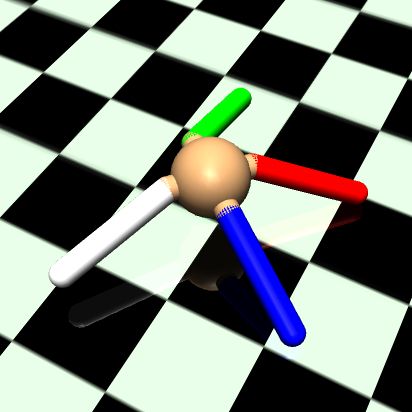
\includegraphics[width=0.4\textwidth]{../img/crop_Basic-Ant.jpg}
    \caption{Robot \emph{StickAnt}}
    \label{imp:fig:robots.StickAnt}
\end{figure}


\paragraph{Robot \emph{AntV3}} \label{imp:robots.Ant}
Jedná se o výchozího robota knihovny \emph{Gymnasium} (ukázka na obrázku
\ref{imp:fig:robots.AntV3})). Morfologie tohoto robota je pokročilejší. Každá
noha má navíc jeden pantový kloub, který můžeme brát jako koleno. Ovládání
tohoto robota již začíná být složitější, kvůli možnosti převrátit se a
spadnout.
\begin{figure}[!htb]
    \centering
    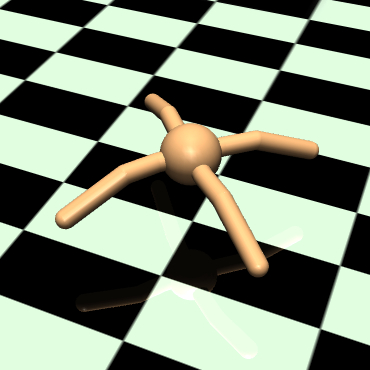
\includegraphics[width=0.4\textwidth]{../img/crop_Ant-v3.jpg}
    \caption{Robot \emph{AntV3}}
    \label{imp:fig:robots.AntV3}
\end{figure}

\paragraph{Robot \emph{SpotLike}} \label{imp:robots.Spot}
Robot inspirovaný pokročilým robotem pojmenovaným \emph{Spot} od firmy
\emph{Boston Dynamics} (popsaný v článku \citep{guizzo2019leaps}). Jedná se o
čtyřnohého robota s morfologií těla, která připomíná psa (ukázka na obrázku
\ref{imp:fig:robots.SpotLike}). Každou nohu ovládají tři klouby (dohromady tedy
12 stupňů volnosti pro celého robota), což z tohoto robota dělá toho
nejobtížnějšího na ovládání. Čtyři vysoké nohy jsou zároveň vratké a tudíž je o
to těžší vyvinout stabilní pohyb, který ho udrží nepadat.

\begin{figure}[!htb]
    \centering
    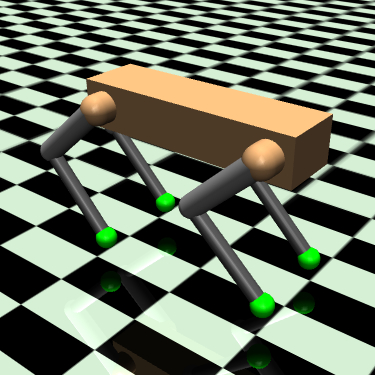
\includegraphics[width=0.4\textwidth]{../img/crop_SpotLike.jpg}
    \caption{Robot \emph{SpotLike}}
    \label{imp:fig:robots.SpotLike}
\end{figure}

\paragraph{}
(Příklady robotů přímo z Gymnasium určených pro neuroevoluci)
\paragraph{Robot \emph{Walker2D}} \label{imp:robots.Walker}

% \begin{figure}[!htb]
%     \centering
%     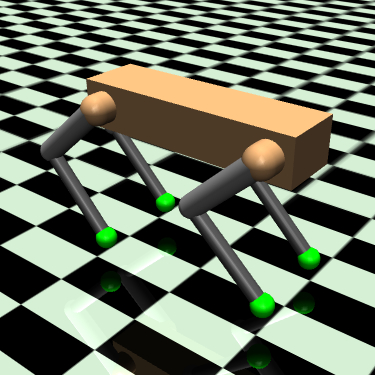
\includegraphics[width=0.4\textwidth]{../img/crop_SpotLike.jpg}
%     \caption{Robot \emph{Walker2D}}
%     \label{imp:fig:robots.Walker2D}
% \end{figure}

\paragraph{Robot \emph{InvertedPendulum}} \label{imp:robots.InvertedPendulum}

% \begin{figure}[!htb]
%     \centering
%     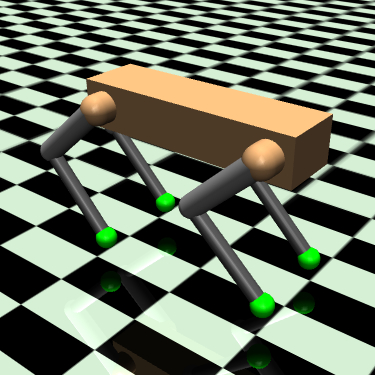
\includegraphics[width=0.4\textwidth]{../img/crop_SpotLike.jpg}
%     \caption{Robot \emph{InvertedPendulum}}
%     \label{imp:fig:robots.InvertedPendulum}
% \end{figure}

\paragraph{Robot \emph{InvertedDoublePendulum}} \label{imp:robots.InvertedDoublePendulum}

% \begin{figure}[!htb]
%     \centering
%     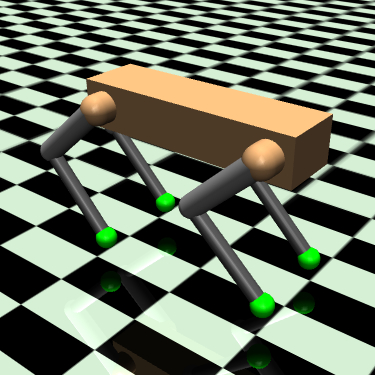
\includegraphics[width=0.4\textwidth]{../img/crop_SpotLike.jpg}
%     \caption{Robot \emph{InvertedDoublePendulum}}
%     \label{imp:fig:robots.InvertedDoublePendulum}
% \end{figure}

\section{Třída experimentů} \label{imp:experimentsetter}
Pro usnadnění vytváření, ukládání a výběru experimentů jsme v modulu
\emph{experiment\_setter} implementovali vlastní jednoduchou třídu
\texttt{Experiments}. Tato třída má za úkol být seznamem nadefinovaných
experimentů, které mohou být rychle načteny buď podle zvoleného názvu
experimentu, nebo podle jména funkce, vytvářející experiment.

Hlavní datovou strukturou třídy je slovník, který má jako klíče názvy
experimentů a jako hodnoty korespondující parametry experimentu (objekt třídy
\texttt{ExperimentParams}). Tento slovník je naplněn v době inicializace třídy
a uživatel do něj může přidat vlastní experimenty (je potřeba vytvořit záznam
ve slovníku experimentů s hodnotou odpovídajících parametrů experimentu).

Třída \texttt{Experiments} obsahuje, všechny experimenty předvedené v této
práci, ze kterých uživatel může brát inspiraci při vytváření vlastních. Samotný
experiment je popsán vždy ve vlastní funkci vracející parametry experimentu.
Jak může vypadat tvorba experimentu můžeme vidět v následující ukázce.

\begin{code}
def exp10_TFS_spotlike(self, run=True):
    robot = robots.SpotLike()
    agent = gaAgents.TFSAgent(robot, ...)
    note = "exp1.0"

    # __create_batch_dir - Funkce, která na základě zvoleného robota, 
    # agenta a zvolené poznámky vytvoří # cestu, kam se uloží 
    # výsledky experimentu.
    batch_dir = self.__create_batch_dir(robot, agent, note) 

    # tvorba parametrů experimentu
    params = ExperimentParams(robot, 
                              agent,
                              ga_population_size=100,
                              ga_generation_count=500,
                              show_best=False,
                              save_best=True,
                              save_dir=batch_dir,
                              note="")

    # pokud je experiment tvořen přímo voláním funkce, vypiš info
    if run: 
        self.__exp_start_note()

    return params
\end{code}

Tato třída výrazně usnadňuje spouštění experimentů pro vstupní prostředí. Navíc
díky dalším metodám (pro kontrolu správného výběru experimentu a pro výpis
všech vytvořených experimentů) má uživatel schopnost pracovat s experimenty,
aniž by měl potřebu znát obsah této třídy.

\section{Grafické rozhraní} \label{imp:GUI}
Pro nastavování a spouštění experimentů může uživatel využít jednoduché
grafické aplikace. Tento přístup je vhodný zejména pro prototypování nápadů na
experimenty. Uživatel v aplikaci může rychle vybírat a měnit parametry jak
agentů, robotů, tak samotného genetického algoritmu. Oproti tomu, použití
grafického rozhraní nemusí být vhodné v případech, že uživatel bude chtít
provádět větší množství předem připravených experimentů, při kterých běh
grafického rozhraní není potřeba.

% TODO: GUI TUI ukázky
TODO: GUI TUI ukázka

\paragraph{Implementace GUI}
Implementace používá modul \emph{PySimpleGUI} \citep{pysimplegui}, umožňující
jednoduchý a rychlý vývoj grafických aplikací pomocí Pythonu. 

\emph{PySimpleGUI} umožňuje vytvářet elementy rozhraní (např.
tlačítka, vstupní textová pole, ale i celá okna) uvnitř vlastních funkcí a
elementy pak vracet jako hodnotu funkce. To oproti jiným grafickým knihovnám
zlepšuje celkovou čitelnost a přehlednost kódu. Elementy musejí být v okně
vložené do rozložení~(\emph{layout}). Tato rozložení ale mohou být jednoduše
uložená v Python seznamech, díky schopnosti Pythonu pracovat se seznamy
heterogenních dat.

Naše grafická aplikace je rozdělená do několika sekcí:

\begin{itemize}
    \item \emph{Main} -- přehled informací o nastavovaném experimentu a
        spouštění experimentu,
    \item \emph{Robot select} -- sekce pro výběr robota,
    \item \emph{Agent config} -- sekce pro výběr a nastavení parametrů agenta,
    \item \emph{Evolution config} -- podrobnější úprava genetických operátorů a
        parametrů evolučního algoritmu.
\end{itemize}

Vytváření jednotlivých sekcí je oddělené do vlastních funkcí, které jsou pak
při inicializaci aplikace volány z rozložení hlavního okna.

Běh aplikace je tak, jak tomu u grafických aplikací bývá, zajištěn nekonečným
cyklem, který se opakuje vždy při příchodu nějaké události do aplikace (např.
kliknutí myší na tlačítko v okně). Modul \emph{PySimpleGUI} pracuje na základě
posílá zpráv o událostech. Tyto zprávy jsou po obdržení zpracovávány uvnitř
nekonečného cyklu a dle potřeby vyřešeny.

Určité sekce využívají napojení na pomocné moduly z centrálního modulu
\emph{RoboEvo} (popsané výše v sekci \ref{imp:roboevo}). Tohoto využíváme
hlavně, abychom umožnili rozsáhlejší modifikace jednotlivých pomocných modulů
(např. popis a nastavování parametrů agenta).

Pokud uživatel spustí vybraný experiment, proběhne proces, ve kterém se z
navolených hodnot v aplikaci vytvoří parametry pro spuštění experimentu (objekt
třídy \texttt{ExperimentParams}), které následně předá modulu \emph{RoboEvo}.
Zároveň se vytvoří nové okno, které vykresluje graf a vypisuje informace o
právě běžícím experimentu. Z tohoto okna může uživatel v libovolný čas zažádat
o prezentaci jedince s dosud nejlepším řešením.

\section{Textové rozhraní} \label{imp:TUI}
Vedle grafického rozhraní lze knihovna ovládat i pomocí zadávání příkazů do
příkazové řádky. Tento přístup ke knihovně se může hodit při vypracování
větších nebo vícero experimentů, kdy očekáváme, že experimenty poběží delší
dobu (několik hodin). Pro tento účel nepotřebujeme a ani by nebylo
nejvýhodnější po celou dobu sledovat okno grafické aplikace.

Textové rozhraní je tedy vytvořené hlavně pro účel spouštění experimentů. Proto
toto rozhraní úzce spolupracuje se třídou experimentů (popsanou výše v sekci
\ref{imp:experimentsetter}). Rozhraní vytváří jednoduchý způsob, jak vybírat a
spouštět vyhodnocení dostupných experimentů.

\paragraph{Ovládání TUI}
Textové rozhraní ovládá uživatel voláním textového rozhraní z příkazové řádky s
různými vstupními argumenty. Těmito argumenty jsou následující:

\begin{itemize}
    \item \texttt{-{}-experiment} -- argument, který obdrží textový vstup
        specifikující jméno jednoho nebo více experimentu (oddělených mezerou),
        jehož parametry chceme načíst a spustit (pracující s modulem
        \emph{experiment\_setter} popsaného v oddíle
        \ref{imp:experimentsetter}),
    \item \texttt{-{}-experiment\_names} -- při výběru tohoto argumentu při
        spuštění programu program vypíše názvy všech dostupných vytvořených
        experimentů z modulu \emph{experiment\_setter} a následně se ukončí,
    \item \texttt{-{}-batch} -- argument číselné hodnoty, specifikující
        kolikrát se má nakonfigurovaný experiment opakovaně spustit (používané
        pro statistické vyhodnocení výsledků experimentů),
    \item \texttt{-{}-batch\_note} -- textový argument umožňující připojit
        vlastní poznámku k názvu složky, do které se experimenty z
        několikanásobného spuštění ukládají (argument nemá žádný efekt pro
        experimenty z modulu \emph{experiment\_setter}),
    \item \texttt{-{}-open} -- textový argument, který obdrží cestu k uloženým
        datům nejlepšího jedince z libovolného předchozího experimentu,
        umožňující vizualizaci řešení daného jedince,
    \item \texttt{-{}-no\_graph} -- argument, který značí, že za běhu algoritmu
        nemá být vykreslován graf průběhu fitness hodnot v
        generacích.
\end{itemize}

\paragraph{Ukázky možných vstupů}
Textové rozhraní úzce spolupracuje s modulem \emph{experiment\_setter}, který
udržuje definované experimenty. Jedním z užitečných parametrů je
\texttt{-{}-experiment\_names}, který TUI nechá vypsat názvy všech definovaných
experimentů.

\begin{code}
>>> TUI.py --experiment_names
<<< List of created experiments:
     - exp10_TFS
     - exp11_TFS_spot
     - exp12_TFS_ant
     ...
\end{code}

Pokud již máme vybraný jeden nebo více experimentů, které chceme spustit,
můžeme je spustit výběrem parametru \texttt{-{}-experiment} a vypsáním seznamu 
zvolených experimentů odděleného mezerou.

\begin{code}
>>> TUI.py --experiment exp11_TFS_spot exp_12_TFS_ant
<<< Starting experiment - exp11_TFS_spot 
    ...
\end{code}

Ve spojení s parametrem \texttt{-{}-experiment} můžeme vybrat další. Těmi mohou
být například parametr \texttt{-{}-batch} (\texttt{-{}-batch 5} bude opakovat
běh všech zvolených experimentů 5krát), nebo parametr \texttt{-{}-no\_graph},
který zabrání průběžnému vykreslování grafů z běhu experimentu.

\paragraph{}
Posledním často používaným parametrem je \texttt{-{}-open}, pomocí kterého
si můžeme v simulačním prostředí přehrát běh nejlepšího jedince ze zvoleného
předchozího experimentu.
\begin{code}
>>> TUI.py --open saved_files/runs/run1/individual.save
<<< (Simulace zvoleného jedince)
\end{code}

\paragraph{Implementace TUI}
Samotná implementace rozhraní je již velmi jednoduchá. Zpracovává uživatelské
vstupy z argumentů, které buď předává dál do korespondujících funkcí, nebo
hlásí a řeší problémy, které mohli při zadávání argumentů nastat.
